%%%%%%%%%%%%%%%%%%%%%%%%%%%%%%%%%%%%%%%%%%%%%%%%%%%%%%%%%
\section{Algoritmo propuesto}
\label{posing:method}
%%%%%%%%%%%%%%%%%%%%%%%%%%%%%%%%%%%%%%%%%%%%%%%%%%%%%%%%%
%\todo{1. Indicar muy brevemente las ventajas de la animación esqueletal alineadas con los objetivos. 2. Indicar porque la técnica clásica no se puede utilizar. La extendemos para anatomía interna. 3. No usamos las técnicas clásicas porque no tiene en cueta la anatomía interna. %2. No entiendo la seguna parte de la frase}
En este apartado, se proponen un conjunto de técnicas capaces de animar la anatomía interna y externa de un paciente virtual. El cauce de animación, que aquí se describe, fue diseñado para trabajar con \emph{\acs{B-rep}s} de los distintos tejidos, aunque dada la flexibilidad del enfoque planteado, posteriormente se extendió a otro tipo de representaciones (ver sec. \ref{posing:animvol}). 
%\todo{
%mete la referencia. Lo he contado por que tú lo haces pero no se si es el mejor sito. 
%Tienes que ir soltando las ideas una a una, no todas a la vez. }
%
%\del{El objetivo es ser capaz de modificar toda la anatomía interna y externa de un modelo anatómico virtual usando una representación superficial. En el mundo de los gráficos por computador, tradicionalmente, se ha utilizado la animación esqueletal para \new{animar modelos articulados}. ????????????????????????????????? Aunque permite una animación de modelos complejos en tiempo interactivo, no tiene en cuenta la relación espacial entre tejidos. Por esta razón, se ha diseñado un cauce basado en la animación esqueletal que se extiende para el uso de representaciones volumétricas.????}
%\todo{%Lo reescribo yo!. Todo esto es muy confuso. 
%No hay un hilo conductor ni una idea clara que vender} 

En el mundo de los gráficos por computador, tradicionalmente se ha utilizado la animación esqueletal para animar modelos articulados, dado que produce resultados visualmente plausibles y son muy eficientes desde el punto de vista computacional. Este conjunto de técnicas se basan en asignar un esqueleto virtual a la representación poligonal de la superficie de un modelo 3D. Es conveniente destacar que un esqueleto virtual no es más que un conjunto jerárquico de huesos virtuales donde los puntos de rotación de cada hueso se definen localmente en el sistema de referencia del padre. 
La idea que subyace bajo esta aproximación es que el número de grados de libertad del esqueleto virtual es muy inferior al número de grados de libertad de la malla superficial. Este tipo de técnicas no pueden aplicarse directamente al problema que se ha enunciado en la sección anterior, puesto que el proceso de animación requiere de la intervención de uno o varios artistas en la preparación de los datos. El resultado final dependerá en gran medida de las destrezas de los artistas implicados en el proceso. 

Tal y como se comenta en la sección \ref{art:animation}, en la bibliografía existen distintas técnicas que buscan automatizar algunas de las etapas de este cauce, pero no están diseñadas para lidiar con modelos que contengan estructuras anatómicas internas. Por consiguiente, en este trabajo de tesis, se propone cómo adaptar el cauce de la animación esqueletal clásica de forma que se pueda aplicar a modelos anatómicos de forma automática. 
%\del{En lugar de utilizar las técnicas clásicas de animación esqueletal, se ha propuesto una nueva manera novedosa de animar anatomías de personajes de manera eficiente, ya que para animar todos los tejidos de forma separada implicaría que habría que realizar las etapas de la animación para cada tejido de manera independiente y que no se podría asegurar que se generaran auto colisiones entre ellos.}

La idea principal que hay detrás del algoritmo propuesto es calcular un campo de desplazamientos continuo a partir del movimiento de los huesos
%\todo{si no es continuo todo lo que dices a continuación no sirve}
en el interior del paciente virtual y utilizarlo para transformar sus estructuras internas. Esto permite deformar los tejidos de forma independiente y, aun así, garantizar que estos se muevan solidariamente, asegurando que no se produzcan colisiones y/o autocolisines, siempre y cuando estos estén muestreados con la suficiente resolución. 
%\del{ solidaria sin necesidad de realizar cálculos independientes y asegurar de esta manera que no se producirá nuevas colisiones.} 
%\todo{cuentalo luego}\del{Además, esta forma de trabajar permite no sólo animar representaciones superficiales, sino que es factible animar modelos volumétricos.}
%\todo{Relata la idea principal. Crear el despalazamiento a partir del movimiento de los huesos. 2. Expliar la diferencia enter hueso virtual y tejido oseo. 3. Una vez acabado el parrafo lee toda esta into para que no haya cosas duplicadas. }
%
De cara a calcular el citado campo de desplazamientos a partir del movimiento del tejido óseo, se discretizará el interior del paciente mediante una malla \emph{Lagrangiana}\footnote{Los marcos de referencia \emph{Lagrangianos} formulan el problema en el sistema de referencia del objeto frente a los \emph{Eulerianos} que formulan el problema en función de una base fija del espacio.}. Después, se calculará la influencia de cada hueso sobre el movimiento de los vértices de la malla \emph{Lagrangiana} y  se utilizará para transformar las representaciones superficiales de los distintos tejidos. 
%\del{La deformación del campo de desplazamientos vendrá dada por el movimiento del tejido óseo. La influencia de uno o un grupo de huesos reales definirá el movimiento del campo y en consecuencia, el del resto de los tejidos mapeados con la representación volumétrica generada a partir de la piel. }
%\todo{Aaron cuida más la redacción. O me pasas cosas más trabajadas o no vamos a acabar nunca!!!.}

Al igual que en la animación esqueletal clásica, esta técnica requiere construir un esqueleto virtual en el que definir las transformaciones que se aplicarán al modelo articulado. Destacar que en el caso que aquí se presenta, esta estructura puede calcularse a partir del tejido óseo del paciente virtual.
%\del{El movimiento del tejido óseo será dirigido por los huesos virtuales. Estos serán creados y ajustados teniendo en cuenta la anatomía real del paciente virtual, construyendo un esqueleto virtual específico. }


%\todo{1. todo automático menos la selección de la pose. 2. Indicar que la animación tradicional confía en el artista en muchos paso. Marcos 2: Este párrafo no explica lo que te pedía. Eso esta explicado antes. Si quieres hablar de la animación hazlo en el paso correspondiente. Pero reescribe este parrafo no esta muy bien. }


Por último, se permitirá al usuario seleccionar la pose del paciente virtual de forma interactiva. Dentro del contexto de esta tesis, el objetivo es permitir que un profesional médico supervise la correcta deformación de los tejidos, con la finalidad de conseguir posiciones útiles para el entrenamiento. Por otra parte, se podrán almacenar posturas predefinidas para automatizar el proceso para futuros modelos anatómicos.


%\del{En la industria, es el animador el que se encarga exclusivamente de los movimientos de los personajes, confiando en sus habilidades???????? """"y del rigging y del pesado""""!!!!!!!!. Otro de los objetivos propuestos para este algoritmo es permitir a un médico dirija y supervise la deformación del paciente virtual de manera interactiva. A su vez, puede guardar posturas interesantes que permitan animar los modelos automáticamente en un futuro.
%Se ha buscado en la bibliografía aquellas técnicas automáticas que puedan ser útiles como se puede leer en el estado del arte (sec. \ref{art:anatomy}) y se han adaptado para ser incorporadas en este método con el objetivo de reducir la interacción del usuario a la selección de pose.""Me cuesta enteder que idea quieres trasmitir""} 
%o dejará la elección de la postura a un profesional médico que supervise la correcta deformación de los tejidos de forma interactiva.


%Como se ha especificado en la sección \ref{posing:req}, esta técnica ha sido diseñada para funcionar con anatomías incompletas siendo sólo obligatorio que la piel y los huesos estén correctamente identificados. \todo{1. Esta frase no se como se enlaza con la anterior. 2. repites la idea de etapas automaticas que ya habías explicado en el paso anterior.}\todo{aqui te quedaste}%El algoritmo propuesto sigue la línea del cauce clásico de animación esqueletal, modificando aquellas etapas con el objetivo de que sea automático y permita modelos incompletos.

%\del{Por tanto, el algoritmo propuestose puede dividir en las siguientes etapas}. 
A continuación, se detallan las etapas en las que se divide el algoritmo (ver Fig. \ref{fig:Resumen}). Tal y como puede comprobarse, muchas de las etapas se inspiran en la animación esqueletal tradicional:
%\todo{Déjalo en ingles, pero en el estado del arte, cuando se hable de rigging, mete un nota al pie donde digas lo que es. Hecho }
\begin{itemize}

	\item \emph{Rigging}: %\todo{Se que has traducido del ingles, pero tio!!! que tu hablas castellano} \del{Un esqueleto virtual predefinido \del{es} ajustado a la anatomía del personaje.}
	en la primera etapa, se adapta un esqueleto virtual a la anatomía del paciente virtual. El algoritmo usa el tejido óseo para calcular el centro de rotación de cada articulación del hueso virtual.
	
     \item \emph{Volumetrización}: en esta etapa, se genera una malla de tetraedros que volumetriza el interior del modelo. Esta malla se genera a partir de la piel y los huesos del paciente virtual y sirve para definir un campo de desplazamientos continuo, que se asociará con el movimiento de los huesos.

    \item \emph{Pesado}: a continuación, se calcula de manera automática la influencia del tejido óseo sobre cada vértice de la malla de tetraedros. 
    
    \item \emph{Mapeado}: se asignan los tejidos a los tetraedros de la malla volumétrica. 

    \item \emph{Selección de pose}: en esta etapa, el movimiento de los huesos virtuales es transferido a la malla de tetraedros, usando una técnica estándar de \emph{skinning}: \ac{LBS}, \ac{DQS} o \ac{COR}. 
    Después, el movimiento de estos tetraedros se transferirá a los vértices de los tejidos del paciente virtual.
    %\del{aplicado a los tejidos del resto del modelo}\todo{Hay algo raro}. 
    Esta etapa puede ser interactiva, dejando al usuario elegir la pose, o pueden usarse otras técnicas de animación (p.ej. \ac{MoCap}) con el objetivo de que la etapa se ejecute de manera automática.%\todo{La cinemática inversa no es automática, es interactiva. }
    \item \emph{Optimización}: de forma opcional, el usuario podrá refinar el resultado obtenido utilizando un método que preserva el volumen del modelo anatómico.
\end{itemize}

%\todo{rehacer imagen resumen}
%\todo{hazla más grande}
\begin{figure*}[!th]
   \centering
    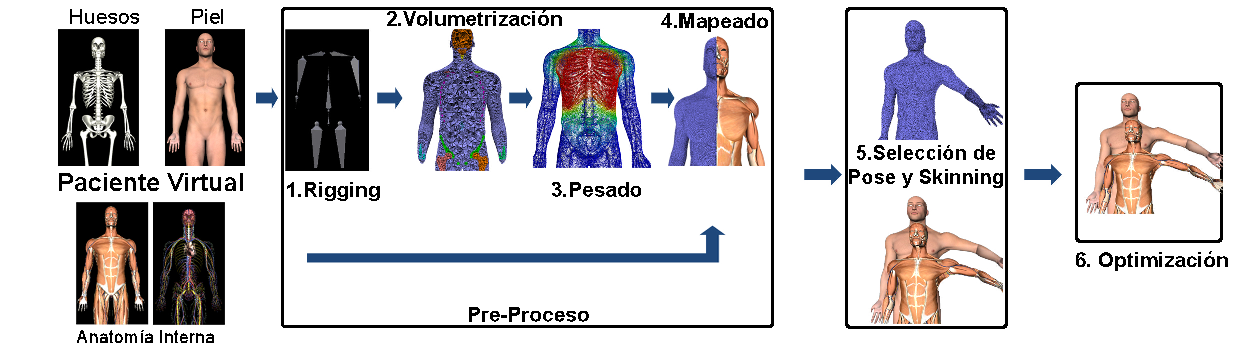
\includegraphics[width=\textwidth]{IMG/resumen.pdf}%[width=0.95\textwidth]
    \caption{Perspectiva general del algoritmo propuesto.}
		\label{fig:Resumen}
\end{figure*}


%

A continuación, se describirá detalladamente cada una de las etapas por separado, remarcando aquellas innovaciones y adaptaciones hechas específicamente en el contexto de este trabajo.



%%%%%%%%%%%%%%%%%%%%%%%%%%%%%%%%%%%%%%%%%%%%%%%%%%%%%%
\subsection{Rigging}
\label{posing:rigging}
%%%%%%%%%%%%%%%%%%%%%%%%%%%%%%%%%%%%%%%%%%%%%%%%%%%%%%
De manera similar a los huesos reales, un esqueleto virtual permite el movimiento del personaje que se quiere animar. El esqueleto virtual está formado por un conjunto jerarquizado de huesos y su posición en reposo se define a partir del sistema de referencia del hueso padre. De esta forma, la transformación que se aplica a cada vértice se expresa localmente en el sistema del coordenadas del hueso al que está asignado.  % \del{Este movimiento puede ser fácilmente ampliable a otros tipos de movimientos más complejos discutidos en la sección \ref{art:rigging}}. 


%\del{De la misma manera, se han mencionado varias formas de crear o ajustar un esqueleto virtual a un modelo de entrada.}

En la bibliografía pueden encontrarse distintas técnicas que permiten automatizar la creación del esqueleto virtual (ver sec. \ref{art:rigging}). Lamentablemente, la mayoría de ellas requieren que el esqueleto virtual esté completamente contenido en los modelos que se desean animar. En el sistema propuesto, todos los pacientes virtuales provienen de registrar un paciente tipo utilizando un modelo de referencia.  De esta forma, se creará un esqueleto virtual tipo y será el algoritmo de registro el encargado de adaptarlo a cada paciente.  %\del{se ha optado por crear un procedimiento por el cual se ajusta un esqueleto virtual predefinido al tejido óseo del paciente virtual. Se utiliza la propia representación superficial del tejido para definir un centro de rotación y los %\todo{muy muy confuso.}
%\todo{
%1. Explica que en la bibliografia existen técnicas que crean en el esqueleto y otras que ajustan uno existente. 
%2. En Rasimas los pacientes se generan registrando datos reales en el modelo del Zygote. 
%3. Redacta lo que viene a  continuación para que este bien ligado con esto. 
%4. Tienes que encuenta que etiquetas el modelo en reposo. %Recuerda el documento que nos pasó antoine. De hecho puedes poner este docuemento en el apendice y citarlo. 
%De verdad falta mucha información}

Con este objetivo, se han identificado manualmente en el modelo de referencia, las regiones significativas de cada hueso o conjunto de huesos, a partir del cual se calculará el sistema local de referencia del hueso virtual. En la figura \ref{fig:humero}, se pueden apreciar las distintas regiones seleccionadas para una muestra de diferentes huesos. 
Las zonas rojas sirven para calcular el centroide que se usará como punto de rotación. Con este punto y los centroides obtenidos de las áreas de color azul y verde, se pueden estimar dos vectores ortogonales: un vector vertical entre la zona roja y verde; y otro horizontal entre la zona verde y azul. El tercer eje se calcula mediante el producto vectorial de ambos. Estos vectores servirán para definir el sistema local de referencia para esa articulación. Para hacer estos cálculos más robustos, el algoritmo considerará (cuando sea posible) regiones grandes, minimizando los posibles defectos de un mal registro. Este proceso es específico para cada hueso virtual y puede ser fácilmente ampliable a otros tipos de huesos o agrupaciones de huesos. La explicación sobre qué zonas se han identificado en este sistema se podrá consultar en el apéndice \ref{anexo:rigging}. 
%
%\del{Estas zonas etiquetadas se identifican en el modelo anatómico de entrada.} 
Inicialmente, en el proyecto \ac{RASimAs}, se utilizó como modelo de referencia a  \emph{ZygoteBody}$^{TM}$, pero se puede asumir que el trabajo realizado puede extenderse a otros modelos de entada.
%\del{ de la herramienta \ac{ITGVPH}. 


Esta etapa concreta ha sido desarrollada en colaboración con el Dr. \emph{Antonie Serruier}, miembro del proyecto \ac{RASimAs} y se ha basado en anteriores trabajos \cite{QUIJANO20131703}.
%\todo{No entiendo esta idea final. Aaron: La idea de como sacar el centro de rotación esta explicada en ese paper}
%\todo{revisar los colores de las fotos}
%\todo{Aumenta el tamño de todas las imágnes}

%\todo{indica el código de colores}
\begin{figure}
   \centering
    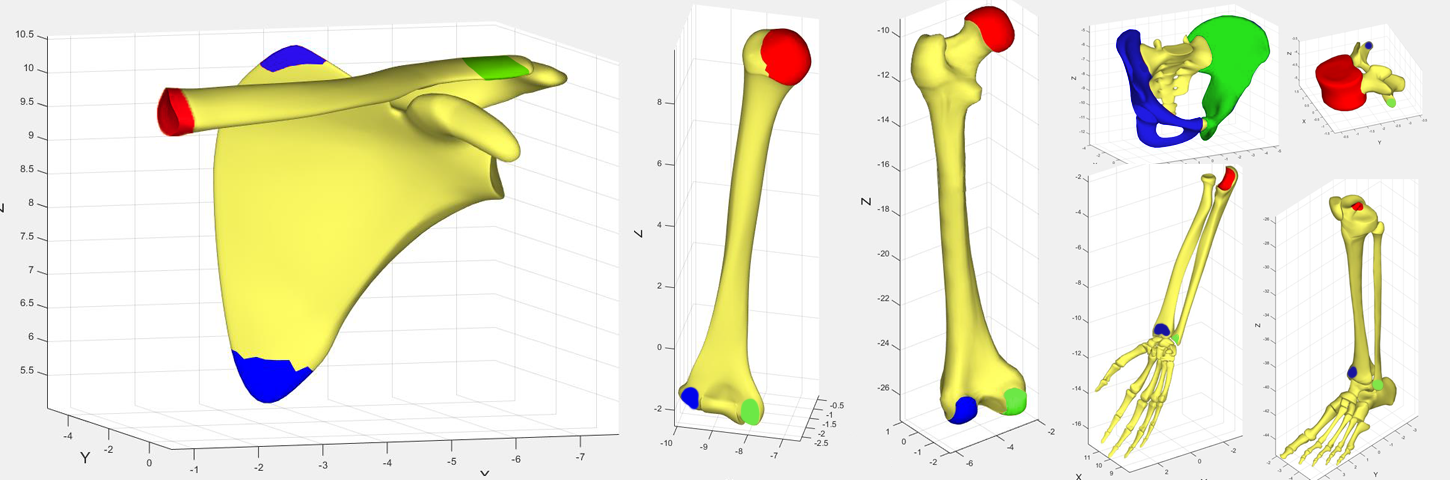
\includegraphics[width=0.95\textwidth]{IMG/rigshoulder.png}%[width=0.8\textwidth]
    \caption{La imagen muestra los huesos del modelo de referencia antes de registrar los datos del paciente. Las áreas coloreadas se utilizan para calcular el sistema de referencia de cada articulación. El centro de rotación se calcula a partir de las zonas rojas. Dos vectores ortogonales se calculan con las zonas azul y verde. El tercer vector ortogonal se calcula en base a los dos anteriores.}
\label{fig:humero}
\end{figure}


%%%%%%%%%%%%%%%%%%%%%%%%%%%%%%%%%%%%%%%%%%%%%%%%%%%%%%
\subsection{Volumetrización}
\label{posing:volumetrizacion}
%%%%%%%%%%%%%%%%%%%%%%%%%%%%%%%%%%%%%%%%%%%%%%%%%%%%%%
%
Como se ha introducido anteriormente, el objetivo es crear un campo de desplazamientos continuo que permita mover la anatomía interna del paciente virtual. El algoritmo discretiza el interior del modelo utilizando la piel y el tejido óseo como referencia, obteniendo una malla volumétrica formada por tetraedros. %\del{Esta malla de tetraedros es una pieza clave del algoritmo que se utilizará para calcular el citado campo de desplazamientos.}
La siguiente etapa (sec. \ref{posing:pesado}) calculará la influencia del movimiento de cada hueso en los vértices de los tetraedros, de forma que el movimiento de los huesos afecte a los vértices de la malla volumétrica. El campo de desplazamientos se obtendrá de forma implícita interpolando el desplazamiento de los vértices en el interior de los tetraedros, mediante el uso de coordenadas baricéntricas. %\del{Esta malla será fundamental en las siguientes etapas.}
%\del{Después, esta malla será donde se calcule el campo de desplazamiento (Sec. \ref{posing:Poses}). También, el campo de desplazamientos guiará la animación del modelo virtual gracias al cálculo del mapeado entre los tetraedros generados en esta etapa y los distintos tejidos (Sec. \ref{posing:Mapeado}).}  \todo{Estas ultimas frases son muy raras, sobretodo la final. Explicas cosas que no son necesarias para esta etapa. }


%\todo{No te das cuenta de confusa que es esta frase. Lo que quieres decir es que no calculas directamente la malla de tetraedros, primero creas una imagen volumétrica. Reescribe}
%\del{En lugar de proceder al proceso de discretización con las representaciones superficiales de los tejidos, se ha optado \new{por} generar una representación volumétrica a partir de la piel y los huesos como paso intermedio para controlar el proceso de discretización y mejorar la robustez del algoritmo. Se genera una imagen en tres dimensiones compuesta por \emph{vóxeles}\footnote{unidad cúbica mínima para representaciones volumétricas} que permitirá simplificar el etiquetado aquellos \emph{vóxeles} que \del{colisionan con} \new{pertenezcan a} la piel y los huesos.}\todo{simplificar?}
La malla volumétrica no se calcula directamente a partir de la representación superficial de los tejidos del paciente. En su lugar, se construye una imagen tridimensional en la que se etiquetan los \emph{vóxeles} que pertenecen a los huesos y la piel del paciente virtual. Este paso intermedio permite controlar el proceso de discretización y mejora su robustez.
%\del{La malla volumétrica no se realiza de forma directa, sino que se ha decidido general una representación superficial a partir de la piel y los huesos como paso intermedio para controlar el proceso de discretización y mejorar la robustez del algoritmo. Se genera una imagen en tres dimensiones compuesta por \emph{vóxeles}}\del{  que permitirá simplificar el etiquetado aquellos que pertenezcan a la piel y los huesos. }
El tamaño de la imagen 3D depende de los tamaños del \emph{vóxel} y de la caja contenedora del modelo. Cuanto más grande sea dicha caja y el tamaño del \emph{vóxel} más pequeño, más detalle tendrá la imagen 3D resultante. Un elevado número de \emph{vóxeles} implicará un mayor consumo de tiempo y memoria.
%\del{Sin embargo, hay que tener en cuenta que a más detalle, más tiempo de cálculo y más consumo de memoria será necesario.}
%\todo{sigue sin gustarme la frase. Piensala más}
Para esta tesis se ha establecido un tamaño de celda que permita tener como máximo una caja contenedora de tamaño 250x700x120 \emph{vóxeles} en todos los modelos probados.

El proceso de \emph{voxelización} comienza etiquetando aquellos \emph{vóxeles} que coinciden con la piel (fig. \ref{fig:voxelizacion}a). Después, los \emph{vóxeles} interiores se etiquetan usando la técnica descrita en \cite{SUZUKI20031} (fig. \ref{fig:voxelizacion}b).
%\todo{expresalo de otra manera}
En este punto, se ha decidido añadir una etapa en la que se eliminan los \emph{vóxeles} marcados como piel (fig. \ref{fig:voxelizacion}c). %\del{donde aquellos \emph{vóxeles} que pertenecen a la superficie de la piel vuelven a estar no etiquetados \del{como vacíos}}. 
Este paso se ha introducido para mejorar la robustez del método en zonas que podrían quedar interconectadas por su proximidad. 
%\todo{No pongas resultados pon la referencia!}
En el apartado \ref{posing:result} se mostrará como esta etapa mejora el resultado final y evita problemas importantes. Finalmente, se procede a etiquetar los \emph{vóxeles} que corresponden a cada hueso como se muestra en la imagen (fig. \ref{fig:voxelizacion}d), de forma similar al procedimiento que se siguió con la piel. 
%
%\todo{puedes hacer la imagenes más grandes. No hay limite de espacio!}
%
\begin{figure}[th]
   \centering
    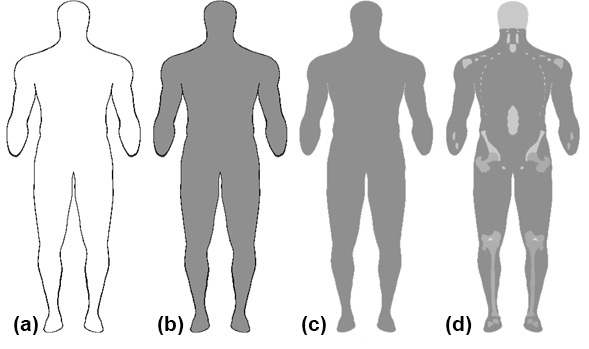
\includegraphics[width=0.95\textwidth]{IMG/Volume2.png}
    \caption{
    Cortes coronales de la imagen volumétrica en las distintas etapas del proceso de \emph{voxelización}.}
\label{fig:voxelizacion}
\end{figure}

%\todo{me gusta esta separación. Usala en el texto. Fase 1 voxelización, fase tetraedrización}
Una vez se ha construido la imagen 3D, esta se utiliza para crear una malla de tetraedros. Para la tetraedrización, se ha utilizado el algoritmo de \ac{RDT} \cite{jamin:hal-00796052}. Este algoritmo permite generar mallas de tetraedros multidominio a partir de mallas superficiales o imágenes 3D. A la hora de configurar el algoritmo, se debía alcanzar un compromiso entre precisión y eficiencia (ver apéndice \ref{anexo:criterios}). En este caso, se ha configurado con la finalidad de incrementar los tetraedros alrededor de la piel y la superficie de los huesos. De esta forma, se ha aumentado la resolución en aquellas zonas donde se requiere calcular la influencia de los huesos de forma precisa.
%permite obtener más detalle en zonas intermedias donde se resolverá la transición de pesos explicado en la siguiente sección.}
%\todo{Explica porque}

En este trabajo, se ha conseguido mantener el número de tetraedros por debajo de $3.5\times 10^6$ y el número de vértices por debajo de $8 \times 10^5$. 
%\todo{Describe la figura }
En la figura \ref{fig:tetra} se puede observar una tetraedrización del modelo \emph{ZygoteBody}$^{TM}$. Los tetraedros del interior del modelo se han coloreado de color morado, mostrando con un color diferente aquellos que pertenezcan a un hueso.
%
\begin{figure}[th]
   \centering
    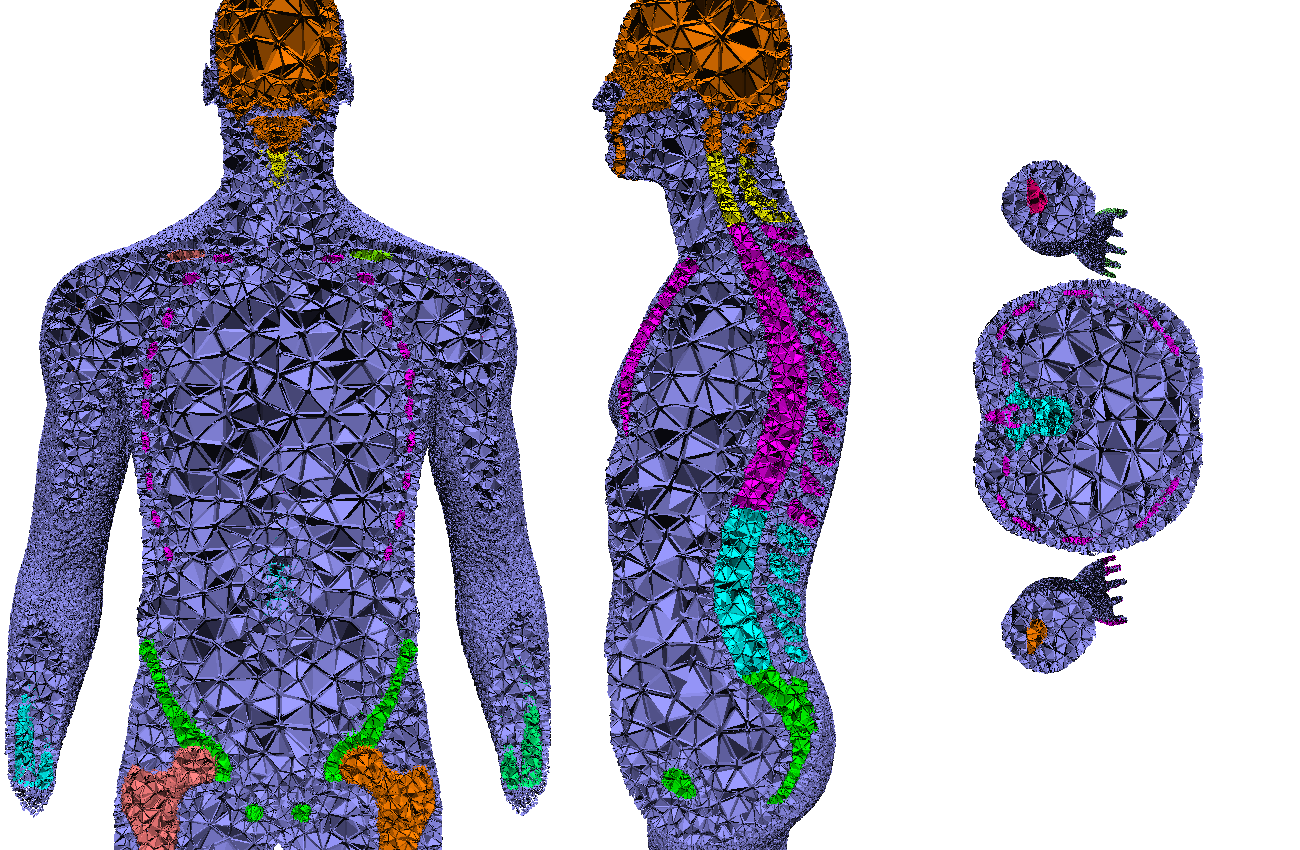
\includegraphics[width=0.95\textwidth]{IMG/boneid.png}
     \caption{Cortes coronales, sagitales y axiales mostrando el resultado de la tetraedrización. Los tetraedros morados representan el interior del modelo, mientras con diferentes colores se muestran los tetraedros etiquetados como hueso.}
\label{fig:tetra}
\end{figure} 
%\todo{Falta el color violeta}

%%%%%%%%%%%%%%%%%%%%%%%%%%%%%%%%%%%%%%%%%%%%%%%%%%%%%
\subsection{Pesado}
\label{posing:pesado}
%%%%%%%%%%%%%%%%%%%%%%%%%%%%%%%%%%%%%%%%%%%%%%%%%%%%%%
%
Como se ha introducido en el estado del arte (ver sección \ref{art:pesado}), la etapa de pesado es donde se calcula como influye el movimiento de cada hueso sobre los vértices de la malla.
Tradicionalmente, esta etapa se realiza de forma manual por un artista ayudado por una herramienta  \ac{CAD}. Aun así, existen técnicas que pueden automatizar el proceso con ciertas restricciones. \emph{Baran y Popovi\'{c}} proponen en \cite{Baran:2007} una técnica de pesado automática donde se asume que el esqueleto virtual tiene forma de modelo de alambre y la malla superficial contiene completamente dicho esqueleto.
%\new{Es habitual encontrar que las técnicas citadas estan orientadas a utilizar mallas superficiales y utilizan una recta como representación del hueso virtual para calcular su influencia en los vértices.

Esta aproximación, no es directamente aplicable al algoritmo presentado, puesto que la mayor parte de la estructuras anatómicas del paciente virtual no contienen al tejido óseo. En esta tesis, se extiende el trabajo de \emph{Baran y Popovi\'{c}} de forma que puedan utilizarse mallas volumétricas en las que el tejido óseo esté etiquetado.  
%\del{Es habitual encontrar que las técnicas citadas están orientadas al pesado en mallas superficiales. Sin embargo, como se están tratando con mallas de tetraedros, hay que adaptar estos modelos a la problemática presente. }

%
%\todo{En el paso anterior no se calculó un campo de desplazamientos. Volumetrizó el espacio interior. El pesado calcula la influencia de los huesos sobre los vértices. Esta influencia se usa para mover los vértices siguiendo el movimiento de los huesos. Una ve que se han movido los vértices se calcula el campo de desplazamientos en el interior de cada tetraedro interpolando mediante coordenadas baricéntricas el desplazamiento de los vértices. En resumen la frase es confusa cambiala}.
%\del{A su vez, tampoco se desea calcular la influencia del esqueleto virtual, sino calcular como se propagan la influencia de los tejidos óseos sobre los demás vértices de la malla de tetraedros.}
%\todo{Piensa un poco más estas dos frases}
%\todo{No entiendo bien la idea}
%\del{Así pues, en este caso se va a calcular la influencia de los huesos reales y no de los huesos virtuales a los vértices de la malla de tetraedros y no de los vértices de los distintos tejidos}
%\todo{Separa las ideas. La primera diferencia es que no se usa el esquelto virtual, sino que se propaga la influencia del tejido oseo. Diferencia 2, no se calcula la influencia sobre el resto de tejidos sino que se calcuala la influencia sobre los vertices de la malla volumetrica}. 

%\todo{Esto es muy raro. Hablas de condiciones que no están en esta este capitulo. No se si se va enteder. Por favor, cuando lo reescribas dedicale tiempo.}

%Se ha tomado como punto de partida la técnica presentada en \cite{Baran:2007}. \emph{Baran y Popovi\'{c}} describen un proceso que realiza el pesado de forma automática, 
La técnica de pesado descrita en \cite{Baran:2007} asume que la influencia de los huesos varia suavemente en la superficie de la malla. Para ello, se propone utilizar la ecuación de la difusión \ref{diffusion}, suponiendo que la influencia de un hueso se propaga como lo haría la temperatura en una superficie. 

%\todo{Transiciones de que. Desarrolla un poco más las cosas}
%\todo{Tanto calor es un poco repetitivo.}

%Existen actualmente técnicas para calcular el pesado de forma más efectiva \cite{Jacobson:2011} comentadas en el estado del arte, pero se basan en el mismo principio\todo{que no se basen en el mismo principio no es suficiente para descartarlas}. 
%Tomando en cuenta la idea original de \emph{Baran y Popovi\'{c}}\cite{Baran:2007}, se ha modificado\todo{que se ha modificado} para adaptarla al algoritmo propuesto debido a que su aplicación no es directa\todo{reescribe la frase}.



%\todo{1. Rehaz la pasiba.}. 
%En \cite{Baran:2007}, se resuelve la ecuación del calor donde se hace una analogía entre temperatura y el peso de los vértices. 
%\todo{Cual es la analogía concreta. Ademas del la difusion del calor hablas en el parrafo anterior. Tienes que hilar mejor las cosas. }
%\todo{Cuando metes una ecuación tienes que explicar los términos. }

\begin{equation}
\label{diffusion}
 \frac{\delta T}{ \delta t} = k \Delta T + q,
\end{equation}
%
donde $t$ es el tiempo, $T$ es la temperatura, $k$ es la conductividad térmica del material
y $q$ son los generadores de calor.
%\todo{revisar}

A la hora de calcular la influencia $Wj$ de cada hueso $j$, se resuelve la ecuación anterior en el caso estacionario: 
\begin{equation}
\label{diffusion1}
 0 =  \Delta W_j +  q_{k}.
\end{equation}
Ahora $q_{k}$ son las zonas de la malla superficial visibles desde el hueso $j$. Estos puntos son fuentes de influencia del hueso $k$. \emph{Baran y Popovi\'{c}} se ven obligados a introducir el término $q_{k}$ para relacionar los puntos de la superficie con el esqueleto virtual. 
%Dado que las condiciones de contorno se imponen directamente sobre la malla de tetraedros, no es necesario definir matrices de visibilidad que transfieran el calor desde los huesos virtuales a los vértices como ocurría en \cite{Baran:2007}. 
En el método propuesto en esta tesis, se dispone de una malla volumétrica del interior del paciente que se utiliza para calcular los pesos $W_j$:  
\begin{equation}
\label{diffusion2}
 0 =  \Delta W_j.
\end{equation}
La ecuación anterior se discretiza espacialmente mediante el \ac{FEM} utilizando la malla volumétrica y las coordenadas baricéntricas de los tetraedros como función de forma (para más información puede consultarse el libro \cite{Lewis2004}):  

\begin{equation}
\label{diffusion3}
 0 =  \mathbf{A} \mathbf{W_j},
\end{equation}
donde $\mathbf{W_j}$ es el vector que contiene la influencia del hueso $j$ sobre todos los vértices de la malla y $\mathbf{A}$ es la matriz de coeficientes del sistema. 
Para poder resolver la ecuación \ref{diffusion3}, se deben establecer las condiciones de contorno del problema en los vértices etiquetados como hueso. De forma que la influencia $w_{i,k}$ del hueso $k$ sobre el vértice $i$ es igual a $1$ si $k=j$ e igual a 0 si
$k \neq j$. Para introducir las condiciones de contorno se ha decidido utilizar la técnica de eliminación: 
\begin{equation}
\label{diffusion4}
 \mathbf{b_j} =  \mathbf{\hat{A}} \mathbf{W_j},
\end{equation}
donde la matriz $\mathbf{\hat{A}}$ se obtiene eliminando las filas y las columnas de los vértices que están etiquetados como hueso y  $\mathbf{b_j}$ es el vector de términos independientes que modela las condiciones de contorno del hueso $j$. Tal y como puede apreciarse en la ecuación \ref{diffusion4} la matriz $\mathbf{\hat{A}}$ es constante para todos los huesos, ya que solo depende de la discretización del dominio. Como esta matriz es simétrica y definida positiva, permite calcular la descomposición de \emph{Cholesky} una única vez y usarla para resolver el sistema lineal de cada hueso.





%\todo{No explicas los términos de la ecuación. antes de hablar de Wj yo hablaria de Wi,j. Por otro lado recuerda que los vectores debería ir en negrita. Deberías intidicar que resuelves la equación en el caso estacionario. Es uno de los motivos de que se simplifique. Cita el libro que uilizamos  }

%De esta forma, se obtiene un campo de pesos $W_j$  para cada hueso donde el tejido óseo correspondiente a $j$  propaga su influencia (temperatura 1) en el que se está resolviendo e influencia nula (temperatura 0) para el resto de huesos.  %de forma que la solución propuesta hace que la energía laplaciana sea estacionaria. Además, esta adaptación asegura una suavidad de orden superior\todo{la frase no suena bien}. 
%\todo{reescribe la frase. Da la sensación que no entiendes que escribes.: flojeo un poco en esta parte sobre todo al escribirla 1 Reformulamos el problemas haciendo cero el laplaciano. Esto es equivalente a minizar la energia. 
%Tienes que hacer un esfuerzo: 
%Ver enlace en comentarios
%https://es.wikipedia.org/wiki/Operador_laplaciano 
%}
%


%Con el objetivo de calcular  de un hueso $j$, se resuelve el caso estacionario definido en la ecuación \ref{diffusion}.%\todo{Tengo la impresion de que sueltas frases sin preocuparte de que sigan un orden logico. Esto está muy flojo.}
%\todo{Lo hablamos en persona. No me gusta la notación}

%A continuación, para calcular los pesos $W_j$, esta ecuación se resuelve para cada hueso $j$, donde se imponen las siguientes condiciones de contorno: se considera que el valor $W_j$ es $1$ (influencia) dentro de los tetraedros etiquetados como $j$; y el valor es $W_j$ es $0$ (influencia 0) dentro de los tetraedros etiquetados como $k$, donde $k$ es cualquier otro hueso que no es $j$. En el equilibrio estático, el resto de vértices tienen que verificar la ecuación \ref{ourdiffusion}. El problema se define de la siguiente manera:

% \begin{equation}
% \label{problema1}
% \Delta W(x)_{j} = 0 \\
% \end{equation}
% \begin{equation}
% \label{problema2}
% W(x)_{j} = 1\ \;
% \forall x \in B_{j} \\
% \end{equation}
% \begin{equation}
% \label{problema3}
% W(x)_{j} = 0\ \;
% \forall x \in B_{k}; k\neq j
% \end{equation}
%\new{donde $W$ es el campo de pesos definido en el dominio $x$. $j$ indica el hueso para el que se está resolviendo, mientras que B es el subdominio de $x$ que representa el hueso real.}

%
%En comparación, a un mayor número de vértices perteneciente a la malla de tetraedros, el sistema de ecuaciones resulta mucho mayor.}
%\new{Con el objetivo de resolver la ecuación \ref{problema1}, se discretiza usando \ac{FEM}  (ver \cite{Lewis2004}). La ecuación \ref{system} muestra la discretización final de la ecuación de difusión:}
%
%\begin{equation}
%\label{system}
%\mathbf{A} \mathbf{W}_j = \mathbf{b}_j,
%\end{equation}
%
%donde $\mathbf{A}$ es la matriz de coeficientes del sistema, el vector $\mathbf{b}_j$ depende de las condiciones de contorno del hueso  $j$ y $\mathbf{W}_j$ es un vector que  contiene los pesos  $w_{i,j}$ para cada vértice sin etiquetar $i$. \new{$\mathbf{A}$ es constante para todos los huesos ya que solo depende de la discretización del dominio. Como esta matriz es simétrica y definida positiva, permite calcular la descomposición de \emph{Cholesky} de esta matriz una única vez y usarla para resolver el sistema lineal de cada hueso.}

Al igual que los algoritmos de pesado clásicos, se deben cumplir las mismas condiciones, \ref{cond1} y \ref{cond2}, que se citan en la sección \ref{art:pesado}. %Es importante mencionar que esta formulación cumple con las restricciones que se imponen en \ref{cond1} y \ref{cond2}. 
Primero, se puede asegurar que el valor máximo y mínimo solo se alcanzan en los huesos (influencia $0$ o $1$).
Segundo, se puede calcular la suma de todos los vectores de pesos resolviendo el siguiente sistema:
\begin{eqnarray}
\sum^{n}_{j=1} \mathbf{\hat{A}} \mathbf{W_j} = \sum^{n}_{j=1} \mathbf{b_j} \\
\mathbf{\hat{A}} \sum^{n}_{j=1} \mathbf{W_j} = \sum^{n}_{j=1}\mathbf{b_j} \\
\mathbf{\hat{A}} \mathbf{W}=\mathbf{b},
\end{eqnarray}
donde $n$ es el número de huesos. Dado que los huesos distintos de $j$ no modifican el valor de ninguna posición del vector $\mathbf{b_j}$ se puede concluir que el vector $\mathbf{b}$ modela un escenario donde todos los huesos tienen un peso de $1$ y por tanto $\mathbf{W}$  tomará el valor $1$ en todas sus posiciones. 


%si se considera \ref{min1}  y  \ref{min2}, donde  $n$ es el número de huesos, el sistema \ref{min3} equivale a calcular los pesos donde todos los puntos del contorno tendrán un valor de $1$. Además, como el máximo y el mínimo valor es alcanzado solamente en el contorno, dará lugar a que el valor de la suma de los pesos $\mathbf{W}$ será $1$, probando la condición \ref{cond2}.
%\todo{Creo que mezclas cosas}


% \begin{equation}
% \label{min1}
% b = \sum^{n}_{j=0} b_{j} 
% \end{equation}
% \begin{equation}
% \label{min2}
% W = \sum^{n}_{j=0} W_{j} 
% \end{equation}
% \begin{equation}
% \label{min3}
% A W = b
% \end{equation}

En trabajos más actuales \cite{Jacobson:2011}, se presentaba una técnica que mejoraba la propuesta de \cite{Baran:2007}, donde se permitía crear puntos de anclaje y cajas contenedoras para controlar la animación del modelo. 
%\todo{lo que has antes de la coma no esta bien enlazado con lo que hay después.}
El inconveniente principal es la complejidad añadida al tener que resolver un problema disperso y cuadrático para imponer las restricciones. Sin embargo, la solución propuesta en esta sección solo requiere resolver un sistema de ecuaciones lineales. 
 %Por otra parte,  mientras que la técnica


%\todo{comprueba la sintaxis, parece cherokee }
 \begin{figure}[ht]
   \centering
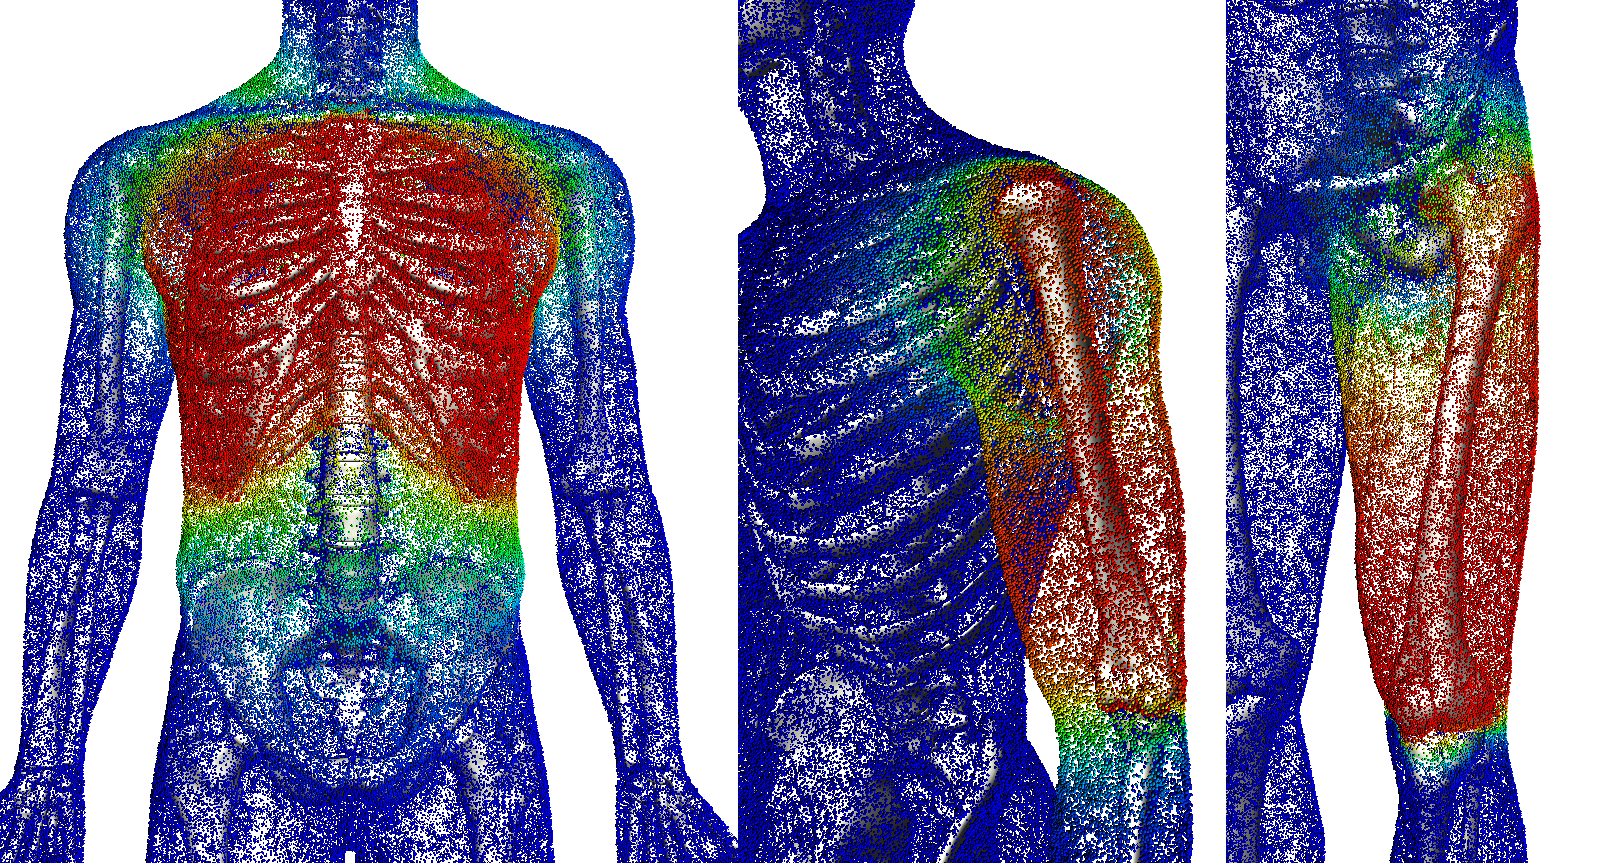
\includegraphics[width=0.9\textwidth]{IMG/weights.png}
     \caption{Influencia de algunos huesos sobre los vértices de la malla de tetraedros. En las zonas con color rojo, los pesos toman valores cercanos a 1 y en las zonas de color azul, los pesos son cercanos a 0.}
      \label{fig:pesado}
\end{figure}
 
La figura \ref{fig:pesado} muestra los resultados obtenidos con el algoritmo propuesto. Se muestra  como ejemplo la influencia de los huesos de la caja torácica, el húmero y el fémur en los vértices de la malla de tetraedros.
%\todo{La idea esta bien pero la redacción es mejorable. Reescribe las dos frases.}

%%%%%%%%%%%%%%%%%%%%%%%%%%%%%%%%%%%%%%%%%%%%%%%%%%%
\subsection{Mapeado}
\label{posing:Mapeado}
%%%%%%%%%%%%%%%%%%%%%%%%%%%%%%%%%%%%%%%%%%
%
Para poder transferir los movimientos de las articulaciones a los tejidos del paciente, hace falta relacionar cada vértice de las mallas superficiales con las que se modela la anatomía con un tetraedro de la malla volumétrica. Para ello, es necesario conocer la posición del vértice en coordenadas del tetraedro en el que recaiga. Así, se calculan sus coordenadas baricéntricas para,  de esta manera, transferir el campo de desplazamientos definido en la malla de tetraedros a los tejidos internos del paciente virtual.
%\todo{Esta frase no suena natural.}




%\new{Para calcular la influencia de los pesos de los teatraedros, se utiliza la posición del vértice que ocupa dentro de su tetraedro. Entonces, se utilizar ayuda de las coordenadas baricéntricas. }
%\todo{??????}
%
%Estas coordenadas indican la influencia de cada uno de los vértices del tetraedro al vértice que esta mapeado.
%Por tanto, hay que calcular cada una de las coordenadas baricéntricas para cada vértice de las mallas superficiales.
%\todo{De verdad que no puedo reescribir nada porque no se lo que quieres decir. Por favor rehaz todo el apartado con cuidado y ligando las ideas.}


Para encontrar el tetraedro que contiene a cada vértice de las mallas superficiales, el enfoque más simple es comprobar cada uno de los $n$ vértices con cada uno de los $m$ tetraedros, 
%
%\todo{La palabra significa suena raro en este contexto. La frase enter es rarr}
aunque este método es muy costoso ($\mathcal{O}(n \cdot m)$). Para acelerar el cálculo global, se ha utilizado la técnica \emph{Spatial Hashing} \cite{Teschner2003}. Esta técnica subdivide el espacio en regiones cúbicas, almacenando en una \ac{tabla hash} solo aquellas regiones que contengan algún tetraedro. El coste de almacenar los tetraedros en la \emph{\ac{tabla hash}} es $\mathcal{O}(m)$. Posteriormente, recorrer la lista de vértices de los distintos tejidos y asignarlos a un tetraedro tiene un coste lineal $\mathcal{O}(n)$, testeando solo los tetraedros que comparten posición en la \emph{\ac{tabla hash}}. Dado que el proceso de volumetrización elimina la piel para evitar ciertos problemas, algunos vértices se encuentran fuera de la malla volumétrica. En estos casos, se busca de forma recursiva en la \emph{\ac{tabla hash}}, el tetraedro más cercano.
De esta manera se ha reducido el tiempo que tarda el método de fuerza bruta de horas a menos de un minuto.


%\todo{No esta bien explicado}


%%%%%%%%%%%%%%%%%%%%%%%%%%%%%%%%%%%%%%%%%%%%%%%%%%%%%%
\subsection{Selección de poses}
\label{posing:Poses}
%%%%%%%%%%%%%%%%%%%%%%%%%%%%%%%%%%%%%%%%%%%%%%%%%%%%%%
%
Otro de los objetivos propuestos para este algoritmo es permitir a un médico dirija y supervise la deformación del paciente virtual de manera interactiva. %A su vez, puede guardar posturas interesantes que permitan animar los modelos automáticamente en un futuro.
En esta etapa, el usuario es el encargado de seleccionar la postura del modelo anatómico. Para ello, el algoritmo propuesto permite usar cinemática directa (fig. \ref{subfig:direct}), poses pregrabadas, animaciones (fig. \ref{subfig:animacion}) e incluso usar el dispositivo \emph{Microsoft Kinect}~\cite{shotton2013} (fig. \ref{subfig:kinect}) para capturar la pose del usuario y transferirla al paciente virtual. Aun así, técnicas como \emph{retargeting} \cite{7581666} o cinemática inversa, podrían añadirse en el futuro. %ser incluidas en el algoritmo.
\begin{figure}[ht]
    \begin{subfigure}[b]{0.32\linewidth}
        \centering
        {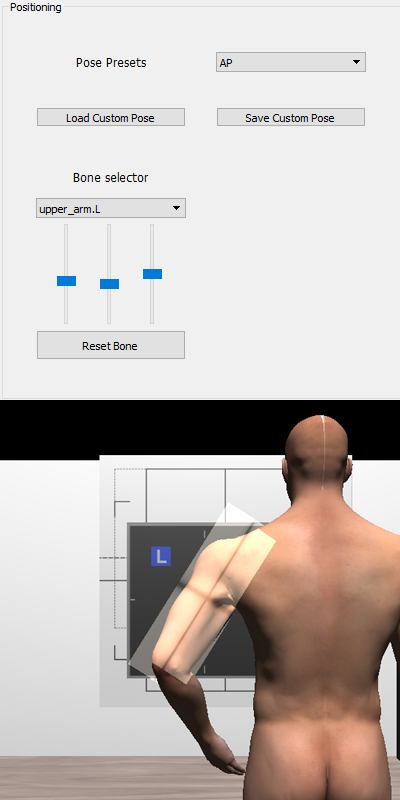
\includegraphics[width=\linewidth]{IMG/Pose1.png}}
        \caption{Posición del brazo izquierdo seleccionada por cinemática directa. \label{subfig:direct}}
    \end{subfigure}
    \null\hfill
     \begin{subfigure}[b]{0.32\linewidth}
        \centering
        {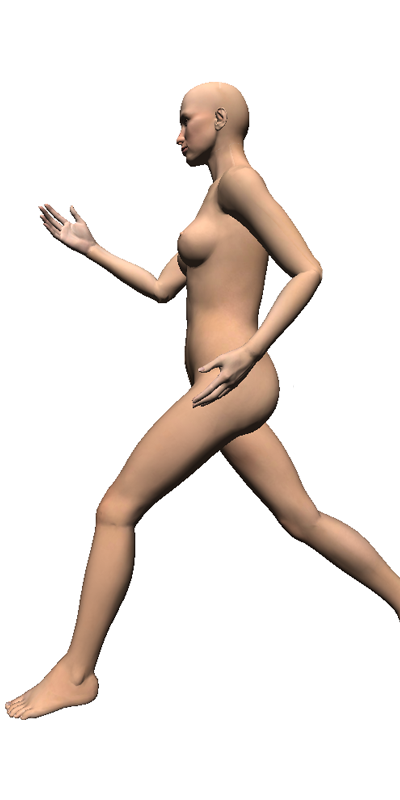
\includegraphics[width=\linewidth]{IMG/Pose3.png}}
        \caption{Extracción de la posición desde un ciclo de carrera. \label{subfig:animacion}}
    \end{subfigure}
    \null\hfill
     \begin{subfigure}[b]{0.32\linewidth}
        \centering
        {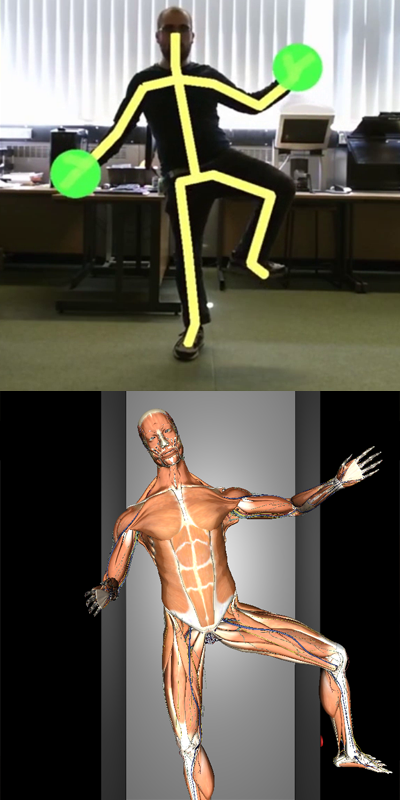
\includegraphics[width=\linewidth]{IMG/Pose2.png}}
        \caption{Selección de pose utilizando la tecnología de \emph{Microsoft Kinect}. \label{subfig:kinect}}
    \end{subfigure}
    \caption{\label{fig:selecpose} Ejemplo del posicionamiento de un paciente virtual.}
   \end{figure}

En la animación esqueletal, para transferir el movimiento del esqueleto virtual a la malla superficial, se pueden utilizar diferentes algoritmos de \emph{skinning} (ver sec. \ref{art:skinning}). %\todo{el skinning no es un modelo matematico, son los algoritmos que transfieren el movimiento de los usos... Tal y como esta redacto parece que en el estado del arte has anticipado que TU ALGORITMO USARA EL SKINNING}.
%En el caso del algoritmo propuesto, se puede tratar los vértices de los tetraedros como vértices de una malla superficial\new{????}. De la misma manera que la animación clásica las animaciones esqueletales son transferidas a la malla volumétrica usando una técnica de \emph{skinning}. Los tetraedros deformados definen un campo de deformación que se utiliza para animar todos los tejidos del paciente virtual.
En el caso del algoritmo propuesto, las técnicas de  \emph{skinning} se aplicarán a los vértices de la malla de tetraedros en lugar de aplicarse directamente a las mallas superficiales. Los vértices del resto de tejidos del modelo serán transformados gracias al campo de desplazamientos definido en la malla volumétrica. Dicho campo se obtendrá de forma implícita interpolando el desplazamiento de los vértices de cada tetraedro en su interior, utilizando coordenadas baricéntricas para trasladar la deformación al paciente virtual. 

%\todo{A partir de ahora solo voy a dar pinceladas. Llevo la mañana del viernes, la del sabado y la del domingo y no avanzo. No puedo comentar cada frase. Es TU RESPONSABILIDAD cuidar la redacción. }


Se ha elegido implementar la técnica de \emph{skinning} descrita en \cite{le2016real},  ya que el método \ac{COR} resuelve algunos de los problemas de \ac{DQS} y \ac{LBS} descritos en la sección \ref{art:skinning}. El algoritmo se basa en calcular, en preproceso, los centros de rotación óptimos para todos los vértices de la malla. %En este caso, es necesario  de tetraedros\todo{paredce que son ellos trabajan con mallas de tetrahedros}. 
Una vez se calcula esta información, el rendimiento del algoritmo es muy similar al de otras técnicas como \ac{LBS} y \ac{DQS}. %Estas tres técnicas son intercambiables entre si debido a que están perfectamente diseñadas para usarse con las arquitecturas gráficas modernas.
Este algoritmo se basa en que los vértices con un pesado similar deben seguir las mismas transformaciones que sus vecinos. En su trabajo, \emph {Le y Hodgins} ~\cite{le2016real} proponen una función de similaridad  $s(\textbf{w}_p,\textbf{w}_s)$ con la que ponderar la contribución de los vecinos según lo parecidos que sean sus pesos:
%\todo{pasivas, intercambiables????}

%\begin{eqnarray}\nonumber
\begin{equation}
\label{similarity}
 s(\textbf{w}_p,\textbf{w}_s) = 
\sum_{\forall i \neq j} w_{p,i}w_{p,j}w_{s,i}w_{s,j}\exp-\frac{(w_{p,i}w_{s,j}-w_{s,i}w_{p,j})^2}{\sigma^2}
\end{equation}
%\end{eqnarray}
\normalsize
%
donde $\textbf{w}_p$ y $\textbf{w}_s$ son vectores de los pesos de los vértices $p$ y $s$, y se realiza la suma para todas las combinaciones de pares de huesos $i$ y $j$ . Por último, $\sigma$ parametriza la función exponencial. 
%\todo{faltan parámetros}
En el estudio que aquí se presenta se ha utilizado un valor de  $\sigma=0.1$. 

La función de similaridad se utiliza posteriormente para calcular el centro de rotación $\textbf{cor}_p$ de cada vértice $p$. En la presente tesis, se ha adaptado la ecuación  propuesta en \cite{le2016real} de forma que pueda utilizarse en mallas volumétricas. Así, la ecuación se quedará de la siguiente manera: 
%
\begin{equation}
%\begin{eqnarray}\nonumber
\textbf{cor}_p = 
\frac
  {
  \sum_{\forall t \in T}
    s(\textbf{w}_p,
      \frac{\textbf{w}_{t1}+\textbf{w}_{t2}+\textbf{w}_{t3}+\textbf{w}_{t4}}{4})
    %\frac{\textbf{v}_{t1}+\textbf{v}_{t2}+\textbf{v}_{t3}+\textbf{v}_{t4}}{4}
    V_t\mathbf{c}_t
  }
  {
  \sum_{\forall t \in T}
    s(\textbf{w}_p,
      \frac{\textbf{w}_{t1}+\textbf{w}_{t2}+\textbf{w}_{t3}+\textbf{w}_{t4}}{4})
    V_t
  } ,
%\end{eqnarray}
\normalsize
\end{equation}
%
donde $\textbf{cor}_p$ es el nuevo centro de rotación del vértice $p$, $t$ es el tetraedro de la malla de tetraedros $T$, $V_t$ es el volumen del tetraedro $t$, $\textbf{c}_t$ es el centroide del tetraedro $t$ y $\textbf{w}_{t1}$, $\textbf{w}_{t2}$, $\textbf{w}_{t3}$ y $\textbf{w}_{t4}$ son los pesos de los vértices del tetraedro $t$. Una vez calculado este centro, se puede usar en la etapa interactiva utilizando el \emph{shader} descrito en \cite{le2016real}.

Finalmente, para animar los vértices de cada malla, el campo de desplazamiento de un punto dentro de un tetraedro se puede calcular interpolando el desplazamiento de cada uno de sus vértices. Se interpola este campo usando las coordenadas baricéntricas de cada tetraedro, ya calculadas en el paso de pesado (sec. \ref{posing:pesado}). Matemáticamente, el campo de desplazamientos calculado es continuo pero no diferenciable dentro de la malla volumétrica y permite calcular una matriz de transformación constante por cada tetraedro (consultar \cite{Muller2004}). Esta matriz de transformación, perteneciente al tetraedro, se aplica a cada uno de los vértices de la malla superficial asociados al tetraedro. Estos cálculos se realizan en la tarjeta gráfica para mejorar el rendimiento del algoritmo.

%\todo{No se si este apartado se entiende lo basta bien. Es muy criptioco. Redactado, a ver que tal}


% %%%%%%%%%%%%%%%%%%%%%%%%%%%%%%%%%%%%%%%%%%%%%%%%%%%%%%
 \subsection{Optimización}
\label{posing:optimizacion}
% %%%%%%%%%%%%%%%%%%%%%%%%%%%%%%%%%%%%%%%%%%%%%%%%%%%%%%
% %

% %

%Los resultados de la etapa previa son visualmente realistas\todo{¿Como lo sabes?}. \ac{COR} reduce el volumen ganado por \ac{DQS} o el volumen perdido por \ac{LBS}\todo{tienes resultados que lo respalden}. Aun así, hay algunos escenarios dónde se produce un cambio apreciable de volumen.El algoritmo propuesto permite al usuario refinar la solución usando un algoritmo basado en físicas
La mayoría de los cauces de animación se basan en transferir el movimiento de un esqueleto virtual a una \acl{B-rep} del personaje mediante un algoritmo de \emph{skinning}. Estos, suelen presentar el problema de garantizar la conservación del volumen. Las pérdidas y ganancias de volumen son comportamientos no deseados, especialmente, teniendo en cuenta que el cuerpo humano está compuesto principalmente por agua, un líquido incompresible. Por este motivo, se ha implementado un paso opcional que optimiza el resultado obtenido en la fase de \emph{skinning}. Esta técnica está basada en la formulación co-rotacional del \ac{FEM}. Cabe destacar que el objetivo de este paso es mejorar la conservación de volumen y no el de simular biomecánicamente el comportamiento de los distintos tejidos. Por este motivo, no se requiere de la caracterización mecánica del paciente virtual.  

%Aunque se haya decidido utilizar un enfoque geométrico para el algoritmo, adicionalmente, se ha propuesto utilizar un modelo basado en físicas que permita al usuario refinar el resultado obtenido. Sin las descripciones mecánicas de los tejidos, se ha propuesto una solución que busca la conservación del volumen de cada tetraedro. Al no disponer de todos los tejidos o de las propiedades mecánicas, el objetivo de esta etapa no es conseguir un solución realista sino, mejorar el aspecto visual del resultado. }

%se puede decir que todos los tejidos están compuestos de agua y se asume que es un fluido incompresible y por tanto, las deformaciones tienen que permitir la conservación de volumen para cada tetraedro.}


%\todo{ponemos fórmulas que tenías en los comentarios?}
%\todo{Si eres capaz de explicarlo...}

El modelo físico utilizado está basado en un modelo mecánico estacionario:
\begin{eqnarray}
\nabla \cdot \mathbf{\sigma} = 0,
\end{eqnarray}
donde $\mathbf{\sigma}$ es el tensor tensión. También, se emplea un modelo elástico isotrópico, homogéneo y lineal:  
\begin{eqnarray}
\mathbf{\sigma} = \mathbf{E}\mathbf{\epsilon}, 
\end{eqnarray}
donde $\mathbf{E}$ es la matriz que define el comportamiento elástico del material y $\mathbf{\epsilon}$ es el tensor de \emph{Cauchy}. Es importante destacar que el tensor de \emph{Cauchy} no está indicado para medir grandes deformaciones.  Debido a su naturaleza lineal, las rotaciones generan distorsiones en la geometría al interpretarlas como deformaciones, produciendo efectos de escalado o abultamientos. Para solucionar esta problemática, se utiliza la formulación co-rotacional del \ac{FEM} para resolver el sistema. La volumetrización del modelo (sec. \ref{posing:volumetrizacion}) se utiliza como discretización espacial y las posiciones de los huesos como las condiciones de contorno necesarias para resolver el problema estático. Para más información se puede consular \cite{Muller2004}.

Con la intención de controlar el modelo elástico planteado, se utilizan los parámetros \emph{ratio de Poisson} y \emph {módulo de Young}. El \emph{ratio de Poisson} controla la conservación del volumen, donde un valor de $0.5$ garantiza su conservación. Sin embargo,  se utiliza un valor ligeramente inferior para asegurar la estabilidad numérica. 
Por otro lado, el comportamiento elástico del material se caracteriza con el valor del \emph {módulo de Young}. Se va a utilizar un material homogéneo, ya que el valor de este parámetro es irrelevante desde el punto de vista teórico y, por tanto, se elegirá su valor con el objetivo de mejorar la estabilidad numérica del sistema. 
Para ello, se ha analizado la matriz de coeficientes del sistema para varios valores del módulo y se ha seleccionado aquel valor que haya maximizado su condicionante.

La formulación co-rotacional calcula las fuerzas internas (aquellas derivadas de la deformación) tras deshacer las rotaciones de cada elemento de la malla. Después, se rotan las fuerzas para ajustarlas a la configuración final del elemento~\cite{Muller2004}. Dado que esta técnica necesita conocer las rotaciones finales que se aplican a cada elemento de la malla, el problema estático se ha de resolver de forma iterativa. Para acelerar la convergencia del algoritmo, se utiliza la deformación seleccionada por el usuario como situación inicial reduciendo  significativamente el número de iteraciones requeridas para llegar a la solución final.  %(ver Fig. \ref{x}). 

Para conocer los desplazamientos de los vértices de la malla de tetraedros se ha formulado un sistema de ecuaciones lineales. Según las propiedades anteriormente citadas, la matriz de coeficientes del sistema lineal es dispersa, simétrica y definida positiva. Este tipo de sistemas de ecuaciones se pueden resolver utilizando el método del gradiente conjugado \cite{Press2007}. La convergencia de estos métodos se acelera con el uso de pre-condicionadores (ver \cite{hauth2003}). En el caso planteado, se utiliza un precondicionador de \emph{Jacobi} y, además, como solución inicial se utiliza la posición del modelo calculada en la etapa de \emph{skinning}. %Para acelerar esta etapa, se utiliza  como solución inicial la posición del modelo ya calculado en la etapa de selección de poses (sec. \ref{posingPoses}), además de emplear un precondicionador de Jacobi.

Finalmente, se utilizarán los desplazamientos de los vértices de los tetraedros para calcular la transformación que se aplicará a todos los tejidos asociados a cada elemento de la malla volumétrica, como se ha detallado en la sección \ref{posing:Poses}.% (ver sec. \ref{posing:Poses}). 

\subsection{Animación de representaciones volumétricas}
\label{posing:animvol}


%\todo{explica el por qué: el campo de desplazamientos, me he traido esto para inspirarme}

Como se puede leer en la sección 
\ref{posing:method}, el algoritmo se basa en el cálculo de un campo de desplazamientos continuo (ver sec. \ref{posing:volumetrizacion}) %\todo{si no es continuo todo lo que dices a continuación no sirve}
en el interior del paciente virtual que permita transformar sus estructuras internas. Esto permite deformar los tejidos de forma independiente y, aun así, garantizar que estos se muevan solidariamente. Se ha decidido deformar los tetraedros y posteriormente interpolar el movimiento a los vértices usando las coordenadas baricéntricas, en lugar de transferir los pesos calculados (ver sec. \ref{posing:pesado}) de los tetraedros a los vértices interiores. 
De esta forma, el campo de desplazamientos definido se puede usar para transformar tanto vértices de representaciones superficiales como \emph{vóxeles} en modelos volumétricos. 


En la figura \ref{fig:volEx} se muestran los pasos para obtener una deformación de una representación volumétrica. En primer lugar, se genera la malla de tetraedros del modelo utilizando la misma técnica explicada en la sección \ref{posing:volumetrizacion}  y se calculan los pesos como se detalló en la sección \ref{posing:pesado}. A partir de esta \emph{tetraedrización}, se definen una serie de \emph{píxeles} dentro de cada tetraedro en la posición deformada. Se mapean con la configuración de reposo utilizando la transformación inversa del campo de desplazamiento. Para ello, se itera sobre cada caja contenedora de la \emph{\ac{tabla hash}} y se utilizan las coordenadas baricéntricas. Este proceso, al ser fácilmente paralelizable en \ac{GPU}, permite que se pueda \emph{renderizar} en tiempo real.


\begin{figure*}[!ht]%[b]%[b!ht]
   \centering
   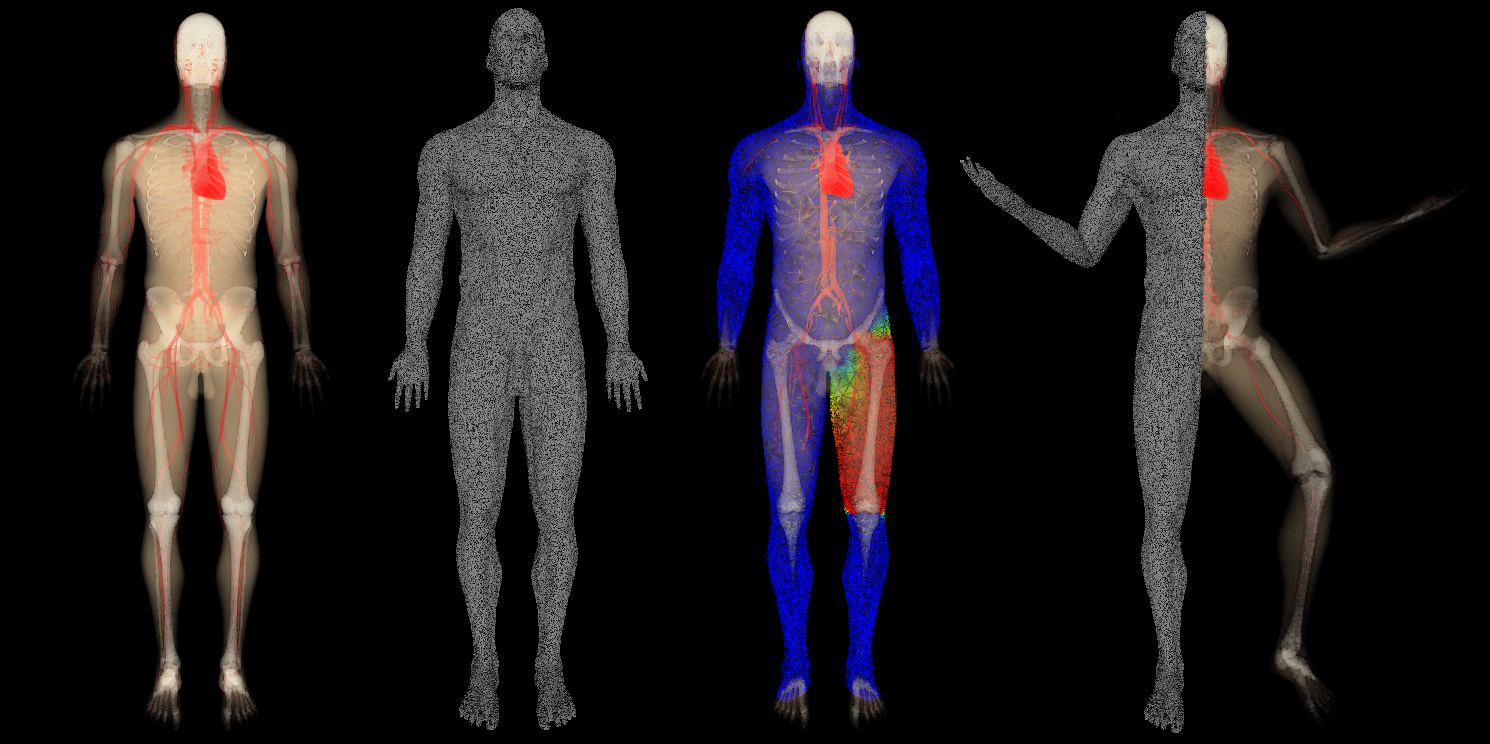
\includegraphics[width=0.90\textwidth]{IMG/Volumetric}
    \caption{Proceso de animación para modelo volumétrico. De izquierda a derecha: (1) modelo volumétrico en reposo, (2) malla de tetraedros generada, (3) malla de tetraedros representando el peso del fémur como ejemplo (rojo significa influencia cerca de 1, azul influencia 0) y (4) malla de tetraedros superpuesta al modelo volumétrico deformado. }
    \label{fig:volEx}
\end{figure*}


%%%%%%%%%%%%%%%%%%%%%%%%%%%%%%%%%%%%%%%%%%%%%%%%%%%%%%%%%
\section{Detalles de implementación}
\label{posing:preprocess}
%%%%%%%%%%%%%%%%%%%%%%%%%%%%%%%%%%%%%%%%%%%%%%%%%%%%%%%%%

Como se puede leer en la sección \ref{posing:req}, la selección de poses debe ser supervisada por un usuario y, por tanto, se debe permitir la animación del modelo de forma interactiva. 
Las etapas de \emph{rigging}, \emph{volumetrización}, \emph{pesado}, \emph{mapeado} y el \emph{cálculo de los centros de rotación} son las etapas más costosas computacionalmente. 
Por este motivo, dado que solo se tienen que ejecutar una única vez por paciente virtual, se puede realizar un preproceso, almacenando los datos auxiliares generados adjuntos al modelo anatómico. 

Para facilitar la interacción, se ha creado una interfaz donde el usuario podrá manipular las articulaciones del paciente virtual, interactivamente y conseguir la transformación del modelo mientras es mostrado por pantalla 

Por último, la etapa de \emph{optimización} no es posible que se ejecute interactivamente. Esto depende del tamaño de la malla volumétrica resultante. Por ello, se deja a elección del usuario cuando se procede a ejecutar esta etapa.


